\chapter{Evaluation}

\section{Multimodal-MNIST}
We first look at applying the anomaly detection pipeline to Multimodal MNIST (MM-MNIST), proposed in \cite{ModDrop}. This dataset consists of the classic MNIST dataset \cite{MNIST} with each image split into quarters, giving four $14\times 14 \times 1$ pixel modalities.\\ 

\subsection{Classifier}
We implement a convolutional neural network with a separate head for each modality, and a tail which combines the head outputs and completes the classification (Table \ref{table:mm-mnist}).\\

\begin{table}[ht]
    \caption{MM-MNIST CNN classifier architecture}
    \centering
    \begin{tabular}{c c}
    \\
    \hline\hline
    \textbf{Layer} & \textbf{Kernel size/units} \\ [0.5ex]
    \hline
    \multicolumn{2}{c}{\textbf{Per-modality heads}} \\
    \hline
    Input & $14\times 14\times 1$ \\
    Dropout & $p=0.2$ \\
    Conv1 & $32\times 5 \times 5$ \\
    Conv2 & $32\times 3 \times 3$ \\
    MaxPool & $2\times 2$\\
    \hline
    \multicolumn{2}{c}{\textbf{Cross modality tail}} \\
    \hline 
    ModDrop & $p=0.1$ \\
    Conv3 & $64 \times 5 \times 5$ \\
    Conv4 & $64 \times 3 \times 3$ \\
    MaxPool & $2 \times 2$ \\
    Fully Connected & $10$ \\
    Log SoftMax & $10$ \\ [1ex] 
    \hline
    \end{tabular}
    \label{table:mm-mnist}
\end{table}
    
ModDrop \cite{ModDrop} is used before the tail to improve robustness to missing modalities as we intend to remove corrupt modalities at this stage. The classifier achieves 97.8\% accuracy on the test set.\\

We use the full GMM method above to generate a baseline for accuracy on corrupted data (Figure \ref{fig:baseline}). Repeated experiments across signal to noise ratio with 0, 1, or 2 corrupted modalities are carried out, and we measure accuracy on both the corrupted data, and the data with corrupted modalities zeroed out.\\

\begin{figure}[H]
    \centering\captionsetup{width=.8\linewidth}
    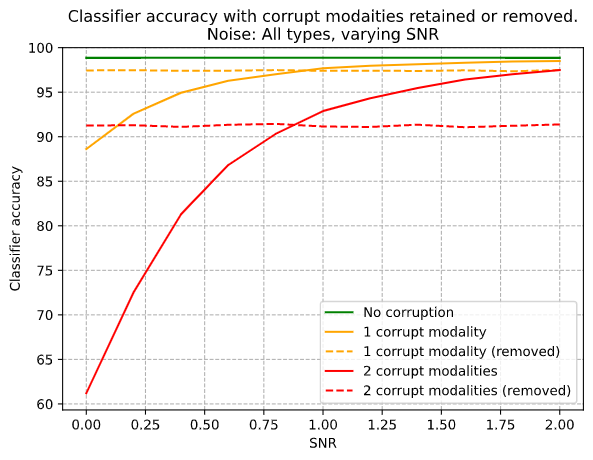
\includegraphics[width=.6\textwidth]{images/classifier_baseline.png}
    \caption{Baseline accuracy for corrupt and subsequently cleaned data with 0, 1 or 2 corrupted modalities. The MM-MNIST classifier appears robust to the noise used above a SNR of around 0.87 with 1 or 2 corrupt modalities. Beyond this threshold accuracy is greater if we don't attempt to clean the data.}
    \label{fig:baseline}
\end{figure}

Figure \ref{fig:baseline} shows that unless a modality contains a high amount of corruption, the modality is still useful for overall classification. Removal of all corruption causes a drop in accuracy under many conditions. The crossover between clean and corrupt modalities in Figure \ref{fig:baseline} has a signal to noise ratio of around 0.87, which in figure \ref{fig:noise} still appears obfuscated to the human eye.\\

As discussed in sections \ref{section:reconstruction} and \ref{chapter:analysis}, attempting to clean each detected modality instead of removing them could make the most of the remaining signal.\\

\subsection{Correlation analysis}
We use the intermediate representations output by the head networks for anomaly detection. The outputs are flattened into 512 element vectors. The networks used in the first stage of DGCCA are fully connected, with layer sizes [512, 125, 64, 32]. These networks are trained on 50000 training samples, with the remaining 10000 held out for corruption detection training. Once the network heads are trained, a linear GCCA is trained on the resulting embeddings to produce transformations to the top $cca\_dim$ canonical variates.\\

Figure \ref{fig:noise_dist} gives an indication of separability of clean and corrupt data. When the amount of noise is high, there is a significant difference between correlations of clean and corrupt data, which suggests easy classification. However, as the amount of noise reduces, correlation and spread both increase and there is more overlap between distributions making classification more difficult. Correlation could also be used as an indicator for how much noise is present, though the usefulness of this may be limited due to the high spread. The distributions also suggest that the Gaussian and feature GMM noise generation methods are more difficult to detect than the more complex GMM methods.\\

\begin{figure}[ht]
    \captionsetup{width=.9\linewidth}
    \begin{subfigure}{.5\textwidth}
      \centering\captionsetup{width=.8\linewidth}
      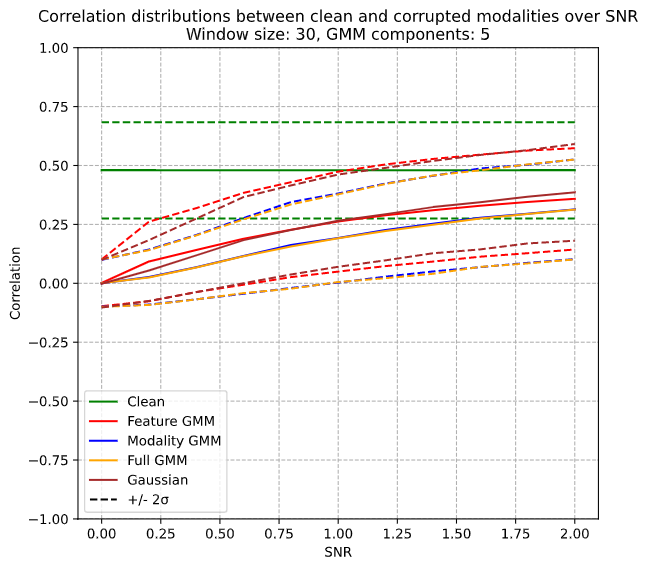
\includegraphics[width=.9\textwidth]{images/noise_dist.png}
      \caption{Distribution of correlations under various types and amounts of noise.}
      \label{fig:noise_dist}
    \end{subfigure}
    \begin{subfigure}{.5\textwidth}
      \centering\captionsetup{width=.8\linewidth}
      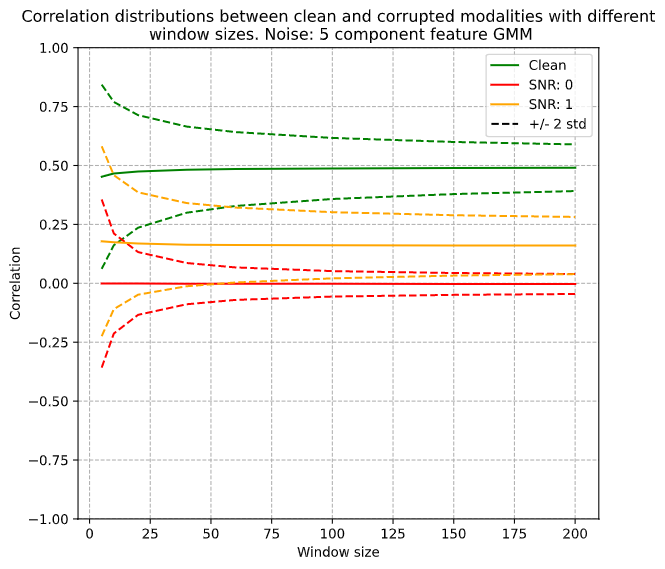
\includegraphics[width=.9\textwidth]{images/window_size.png}
      \caption{Distribution of correlations as window size increases.}
      \label{fig:window_size}
    \end{subfigure}
    \caption{Distribution of correlations under different noise and sample size conditions.}
    \label{fig:noise_separability}
\end{figure}

Varying the number of samples used to calculate correlation could reduce spread of correlation distributions and increase separability. Figure \ref{fig:window_size} shows the spread of correlations reducing with when more samples are used. Increasing the number of samples is not always desirable, as for real-time tasks waiting for a large number of undetected corrupt samples to be collected is not always possible.\\

For remaining experiments a sample size of 30 is used as it gives a reasonable balance of correlation spread and detection latency.\\

\subsection{Anomaly detection}
The remaining 10000 elements of the training set are used for training the pairwise correlation thresholds. Correlations between DGCCA embeddings for each pair of modalities are measured on clean data and on data that has been corrupted with noise. Figure \ref{fig:pairwise_acc} shows accuracy of pairwise corruption detection using various threshold methods. The best performing method is intersection, having higher accuracy in general than percentile methods. The best performing percentile is 0.05, having slightly lower accuracy than the intersection method.\\

Figure \ref{fig:modality_acc} gives modality corruption detection accuracy using the same threshold methods. We see that as SNR increases, the accuracy of the percentile threshold method rises above that of the intersection threshold method. The number of pairwise false negatives is fixed when using the percentile threshold method, so a reduction in accuracy over SNR is purely dependent on an increase in false positives. For the intersection method, both false positives and false negatives increase with SNR. This suggests that false negatives during the pairwise classification stage have a greater negative impact than false positives on overall modality detection accuracy.\\

\begin{figure}[ht]
    \captionsetup{width=.9\linewidth}
    \begin{subfigure}{.5\textwidth}
      \centering\captionsetup{width=.8\linewidth}
      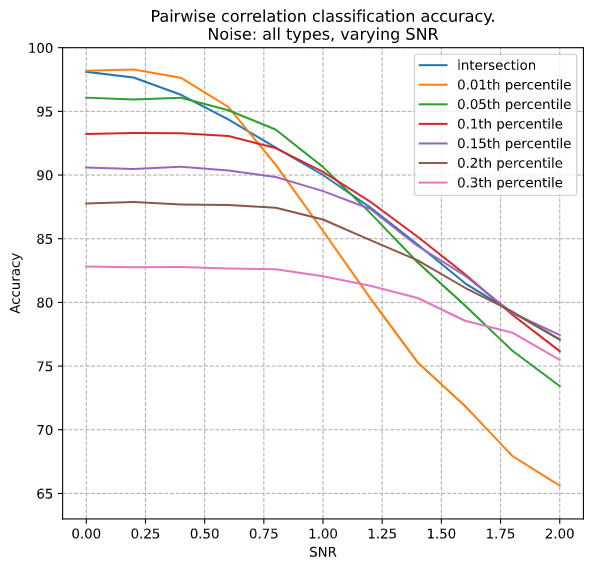
\includegraphics[width=.9\linewidth]{images/pairwise_acc.png}  
      \caption{Pairwise corruption detection accuracy.}
      \label{fig:pairwise_acc}
    \end{subfigure}
    \begin{subfigure}{.5\textwidth}
      \centering\captionsetup{width=.8\linewidth}
      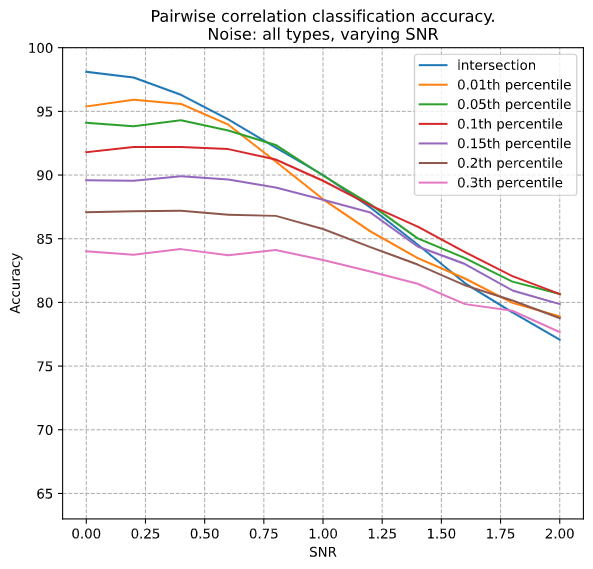
\includegraphics[width=.9\linewidth]{images/modality_acc.png}  
      \caption{Modality corruption detection accuracy.}
      \label{fig:modality_acc}
    \end{subfigure}
    \caption{Comparison of pairwise and modality corruption detection accuracy over different threshold generation methods.}
    \label{fig:threshold_method}
\end{figure}

In addition to limiting of false negatives, the percentile threshold method does not require knowledge of the type of noise that will be encountered. In figure \ref{fig:threshold_method}, the intersection classifier is trained by generating noise of the specified SNR, whilst the percentile method requires no noise during the entire training pipeline. This may make the percentile method more useful in real world scenarios where obtaining corrupt data may not be practical.\\

For remaining experiments, the 0.05th percentile classifier is used for pairwise corruption detection.\\

Figure \ref{fig:mod_classifiers} shows that the delta classifier gives significant accuracy gains over the proportional classifier using the 0.05 percentile threshold method, supporting the idea that correlation can be used as an indicator for quantity of noise, especially when we have correlations from multiple pairs. Although accuracy of both methods drops significantly as SNR increases, Accuracy in the worst tested case is still greater than 80\%.\\

\begin{figure}[H]
    \centering\captionsetup{width=.8\linewidth}
    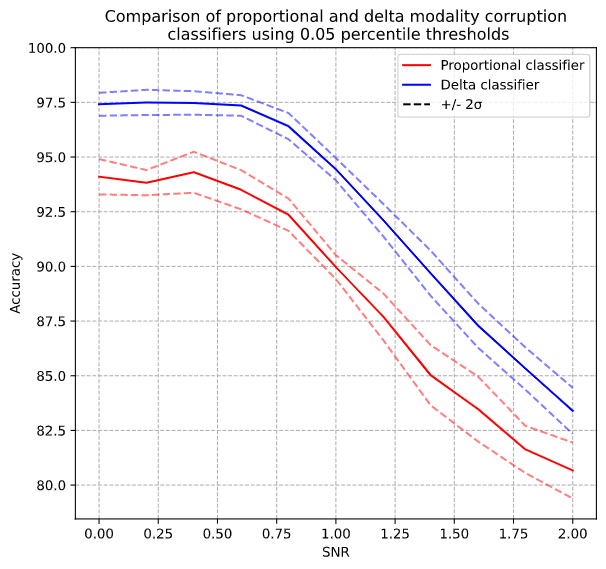
\includegraphics[width=.6\textwidth]{images/modality_classifiers.png}
    \caption{Proportional and delta corruption classification methods.}
    \label{fig:mod_classifiers}
\end{figure}

\subsection{Modality cleaning}
An overall goal of this project is to reduce the impact corruption has on the multimodal network. To remove corruption, modalities identified as corrupt are replaced with zeros before being fed to the tail of the MM-MNIST classifier. Use of ModDrop as the first layer of the tail should make the classifier robust to modality removal at this stage, though performance is still expected to suffer if otherwise useful data is removed.\\

Classifier accuracy is compared on data with no modalities removed, known corrupt modalities removed, and modalities identified by the anomaly detection pipeline removed. Figure \ref{fig:005_delta_results} shows accuracy across a range of noise. \\

\begin{figure}[ht]
    \captionsetup{width=.9\linewidth}
    \begin{subfigure}{.5\textwidth}
      \centering\captionsetup{width=.8\linewidth}
      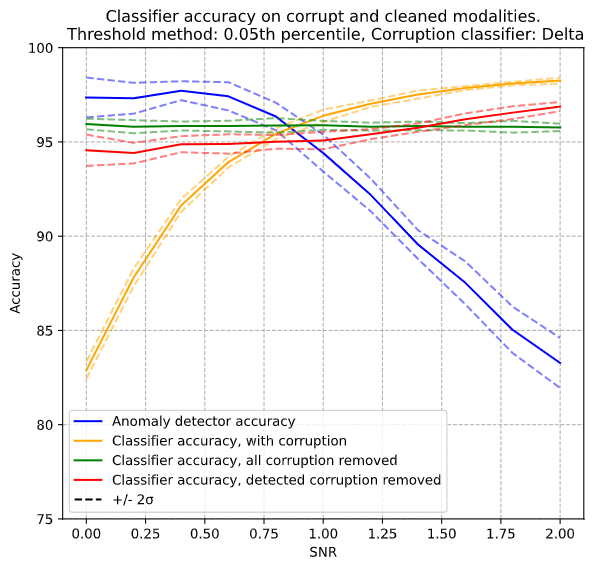
\includegraphics[width=.9\linewidth]{images/005_delta_results.png}  
      \caption{Performance of anomaly detector and MM-MNIST classifier on corrupted and cleaned data using the best found anomaly detector.}
      \label{fig:005_delta_results}
    \end{subfigure}
    \begin{subfigure}{.5\textwidth}
      \centering\captionsetup{width=.8\linewidth}
      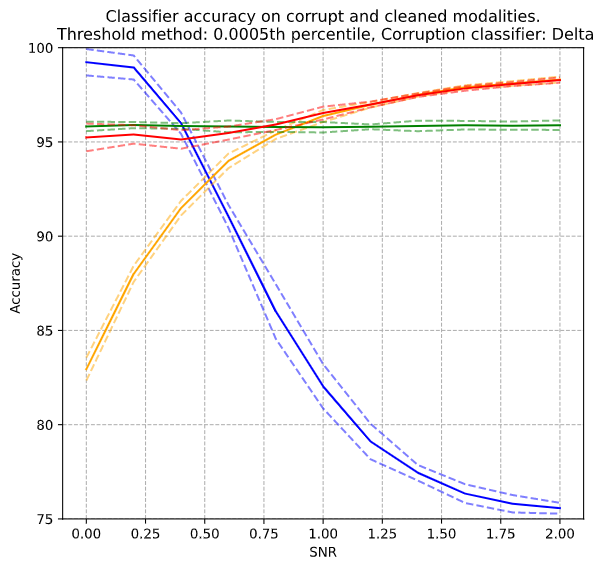
\includegraphics[width=.9\linewidth]{images/00005_delta_results.png}  
      \caption{Performance of anomaly detector and MM-MNIST classifier on corrupted and cleaned data using a lower percentile threshold.}
      \label{fig:00005_delta_results}
    \end{subfigure}
    \caption{Classifier results on corrupted and cleaned data using two different anomaly detector specifications.}
    \label{fig:performance_results}
\end{figure}

With higher amounts of noise, the anomaly detector clearly improves classifier performance when compared to classifying using the corrupted data, with an accuracy increase of 11.6\% when no signal is present. However, as the SNR increases classifier performance on the raw data exceeds that of the clean data, even when cleaned with a theoretically perfect classifier. The drop in accuracy resulting from cleaning the data with the anomaly detector is 1.3\% with an SNR of 2. It is expected that in the real world modalities will be clean most of the time, so this essentially limits overall classifier accuracy.\\

The approach taken so far has been to maximise anomaly detector accuracy. Given the high classification accuracy on corrupted data above the sensitivity threshold, it is beneficial to allow certain amounts of corruption through to the classifier, which necessarily reduces anomaly detector accuracy.\\

Notice that the raw data (yellow) can be seen as having been cleaned by an anomaly detector with no false negatives, no true negatives, and many false positives. The perfectly cleaned data (green) has been cleaned by an anomaly detector with no false negatives or false positives. This suggests that for SNRs above the classifier sensitivity threshold, anomaly detector false positives are in fact beneficial, and provided an anomaly detector returned no false negatives it would result in an accuracy somewhere between the two. As the anomaly detector cleaned classifier accuracy is lower than the perfectly cleaned accuracy for some values above the sensitivity threshold, it suggests that the false negative rate of the anomaly detector is too high.\\

The anomaly detector has a false negative rate of 2.2\%, higher than the $\approx 1\%$ disparity between raw and cleaned data close to the classifier sensitivity threshold. Since the anomaly detector false negative rate is influenced by the pairwise threshold classifier, and the percentile threshold method used essentially allows the pairwise false negative rate to be selected, it is expected that a lower percentile would result in a higher classification accuracy for noise above the sensitivity threshold.\\

Figure \ref{fig:00005_delta_results} gives performance for the best found percentile threshold of 0.0005. 

\begin{table}[ht]
    \centering
    \caption{Anomaly detector classifier comparison. Threshold method: 0.0005 percentile, Classifier: Delta, Noise: All}
    \begin{tabular}{c c c c c c c c c c c c}
    \hline\hline
    & \multicolumn{10}{c}{\textbf{SNR}} \\
    \hline
    & 0.0 & 0.2 & 0.4 & 0.6 & 0.8 & 1.0 & 1.2 & 1.4 & 1.6 & 1.8 & 2.0 \\
    \hline\hline
    \textbf{Best accuracy} & 95.2 & 95.4 & 95.1 & 95.5 & 95.9 & 96.5 & 97.0 & 97.5 & 97.8 & 98.1 & 98.2 \\
    \textbf{vs. corrupted} & 12.3 &  7.4 & 3.6 & 1.5 & 0.5 & 0.2 & 0.0 & 0.0 & 0.0 & 0.0 & 0.0 \\
    \textbf{vs. cleaned} & -0.5 & -0.5 & -0.7 & -0.4 & 0.1 & 0.8 & 1.2 & 1.6 & 2.0 & 2.2 & 2.4 \\
    \hline
    \end{tabular}
    \label{table:classifier_results}
\end{table}

